% This example is meant to be compiled with lualatex or xelatex
% The theme itself also supports pdflatex
\PassOptionsToPackage{unicode}{hyperref}
\documentclass[aspectratio=1610, 9pt]{beamer}

% Load packages you need here
\usepackage{polyglossia}
\setmainlanguage{german}

\usepackage{csquotes}


\usepackage{amsmath}
\usepackage{amssymb}
\usepackage{mathtools}

\usepackage{hyperref}
\usepackage{bookmark}
\usepackage{siunitx}

\usepackage{tikz}
\usetikzlibrary{positioning,tikzmark}
% load the theme after all packages

\usetheme[
  showtotalframes, % show total number of frames in the footline
  % dark, % optional dark theme, uncomment to use
]{tudo}

% Put settings here, like
\unimathsetup{
  math-style=ISO,
  bold-style=ISO, nabla=upright,
  partial=upright,
  mathrm=sym,
}

\title{Upper Limits\includegraphics[width=0.1\textwidth]{logos/applogo_unofficial_rainbow.pdf}}
\author[S.~Fröse]{Stefan Fröse}
\titlegraphic{
\includegraphics[height=0.6\textheight]{imgs/null_hypothesis.png}}


\begin{document}

\maketitle

\begin{frame}{Introduction}
    \begin{minipage}{0.49\textwidth}
        \Large
        \textbf{Dark matter upper limits:}
        \begin{itemize}
            \item Blue dots: UL from data
            \item Central blue line: median from simulations
            \item Green $\pm 1\sigma$ from simulations
            \item Yellow $\pm 2\sigma$ from simulations
        \end{itemize}
    \end{minipage}
    \hfill
    \begin{minipage}{0.5\textwidth}
        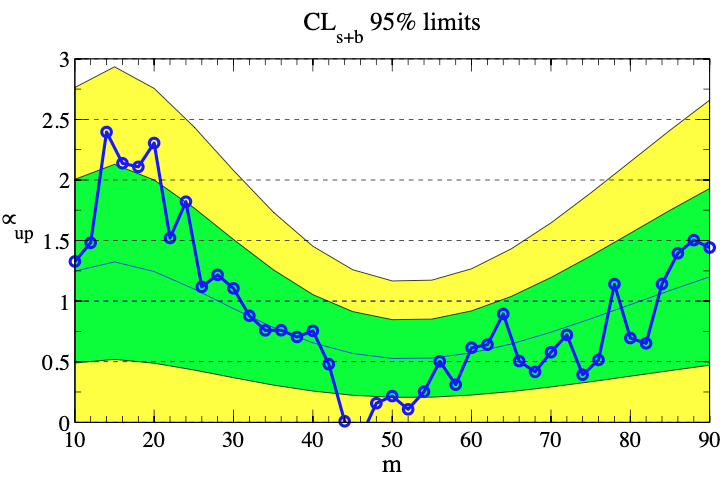
\includegraphics[width=0.8\textwidth]{imgs/CL up.png}
    \end{minipage}
\end{frame}



\begin{frame}{Experiment}
    \centering
    \Large
    \begin{align}
        &\mathcal{L}(\mu,b) = \frac{(\mu s + b)^{N_\text{ON}}}{N_\text{ON}!} e^{-(\mu s + b)} + \frac{(\tau b)^{N_\text{OFF}}}{N_\text{OFF}!} e^{-\tau b} \notag \\[4ex]
        \mu &= \text{strength parameter} \notag \\
        s &= \text{signal counts from model} \notag \\
        b &= \text{background counts from model}\notag 
    \end{align}
\end{frame}


\begin{frame}{Test statistic}
    \begin{minipage}{0.49\textwidth}
        \Large
        \centering
        \begin{align}
            q_\mu = -2 \log{\frac{\tikzmarknode{nullhypo}{\mathcal{L}}(data\vert\mu,\hat{b}_\mu)}{\mathcal{L}(data\vert\hat{\mu},\hat{\hat{b})}}} \notag 
        \end{align}\\[3ex]
        \begin{tikzpicture}[overlay, remember picture,node distance=0.5cm]
            \node (descr) [above right=0.5cm and 0.5cm of nullhypo]{\textbf{Null hypothesis}};
            \draw[tuorange,->,thick] (nullhypo) to [in=180,out=90] (descr);
        \end{tikzpicture}
        $\Rightarrow$ Profiled log-likelihood ratio (pLLR)
        \begin{align}
            p = \int_{q_\mu^\text{obs}}^\infty f(q_\mu\vert \mu,\hat{b}_\mu)\,\mathcal{d}q_\mu \notag
        \end{align}
        p-value: Probability that result at least as extreme as observed result under true null hypothesis $\rightarrow$ small p-value means very unlikely under null hypothesis
    \end{minipage}
    \hfill
    \begin{minipage}{0.5\textwidth}
        \includegraphics[width=\textwidth]{build/distribution.pdf}
    \end{minipage}
\end{frame}

\begin{frame}{Significance}
    \begin{minipage}{0.49\textwidth}
        \Large
        Wanted: Reject null hypothesis only background
        \centering
        \begin{align}
            \mu &= 0 \notag \\
            p &= \int_{q_0^\text{obs}}^\infty f(q_0\vert 0,\hat{b}_0)\,\mathcal{d}q_0 \notag
        \end{align}
    $\rightarrow$ small p-value means: background only is very unlikely
    \end{minipage}
    \hfill
    \begin{minipage}{0.5\textwidth}
        \includegraphics[width=\textwidth]{build/distribution.pdf}
    \end{minipage}
    \centering
    \Large
    $\Rightarrow$ Calculate significane from p-value
\end{frame}

\begin{frame}{Upper Limit}
    \begin{minipage}{0.49\textwidth}
        \Large
        Wanted: Reject specific $\mu = \mu_\text{UL}$\\
        \centering
        \begin{align}
            p &= \int_{q_{\mu_\text{UL}}^\text{obs}}^\infty f(q_{\mu_\text{UL}}\vert \mu_\text{UL},\hat{b}_{\mu_\text{UL}})\,\mathcal{d}q_{\mu_\text{UL}} \notag
        \end{align}
        $\rightarrow$ Confidence level (CL) of \SI{95}{\percent} $\Rightarrow p = 1-\text{CL}$ 
    \end{minipage}
    \hfill
    \begin{minipage}{0.5\textwidth}
        \includegraphics[width=\textwidth]{build/distribution.pdf}
    \end{minipage}
    \centering
    \Large
$\Rightarrow$ Find $\mu^{\SI{95}{\percent}}_\text{UL}$ for which the probability of mistakenly rejecting the hypothesized $\mu^{\SI{95}{\percent}}_\text{UL}$ is less or equal to $\SI{5}{\percent}$\\
    $\Rightarrow$ $\SI{95}{\percent}$ equal to beeing significant with more than $2\sigma$
\end{frame}

\begin{frame}{Problem}
    \Huge
    \centering
    \textcolor{tuorange}{We need to know $f(q_\mu\vert \mu,\hat{b}_\mu)$}
\end{frame}


\begin{frame}{Asimov Dataset}
    \Large
    \begin{itemize}
        \item \textbf{Solution 1:} Generate a lot of toy datasets to compute $f(q_\mu\vert \mu,\hat{b}_\mu)$
        \item \textbf{Solution 2:} Use Wald's take on the approximation $\rightarrow$ $\chi^2$ distributed \\
            \begin{align}
                -2\log{\lambda(\mu)} = \frac{(\mu-\hat{\mu})^2}{\sigma^2} + \mathcal{O}(1/\sqrt{N}) \notag
            \end{align}
    \end{itemize}
    $\Rightarrow$ Gaussian distributed! But how do we find $\sigma$? $\Rightarrow$ Asimov dataset
\end{frame}

\begin{frame}{Asimov Dataset}
    \Large
    \begin{itemize}
        \item Generate dataset where the expected counts are equal to the measured counts
        \item Calculating the estimators of the dataset obtains the true parameters
        \item $n_i = E[n_i] = \mu^\prime s_i + b_i$
        \item Asimov likelihood: \\
            \begin{align}
                \lambda_A = \frac{\mathcal{L}(\mu,\hat{b}_\mu)}{\mathcal{L}(\hat{\mu},\hat{b})} = \frac{\mathcal{L}(\mu,\hat{b}_\mu)}{\mathcal{L}(\mu^\prime,b)} \notag
            \end{align}
        \item Find $\sigma$:\\
            \begin{align}
                V^{-1}_{jk} = -E\left[\frac{\partial^2 ln\mathcal{L}}{\partial\theta_j\partial\theta_i}\right] = -\frac{\partial^2 ln\mathcal{L}_A}{\partial\theta_j\partial\theta_i} \notag
            \end{align}
    \end{itemize}
\end{frame}

\begin{frame}{Distribution}
    \Large
    \centering
    \begin{minipage}{0.49\textwidth}
        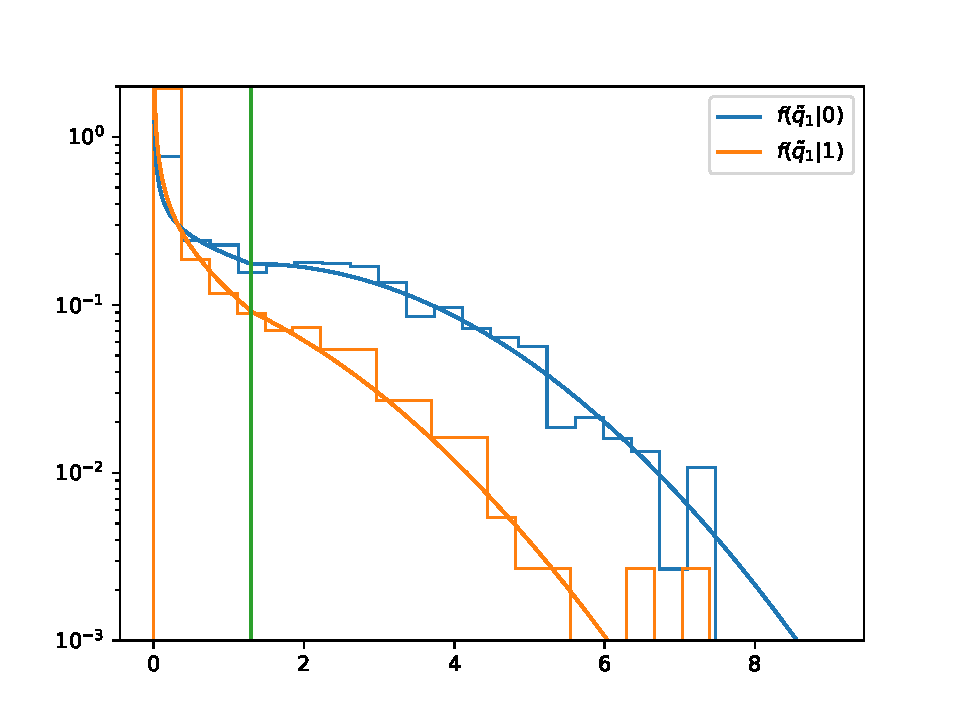
\includegraphics[width=\textwidth]{plots/paper_plot.pdf}
    \end{minipage}
    \hfill
    \begin{minipage}{0.5\textwidth}
        \includegraphics[width=\textwidth]{imgs/distribution.png}
    \end{minipage}
\end{frame}

\begin{frame}{Median}
    \Large
    \centering
    \begin{minipage}{0.49\textwidth}
        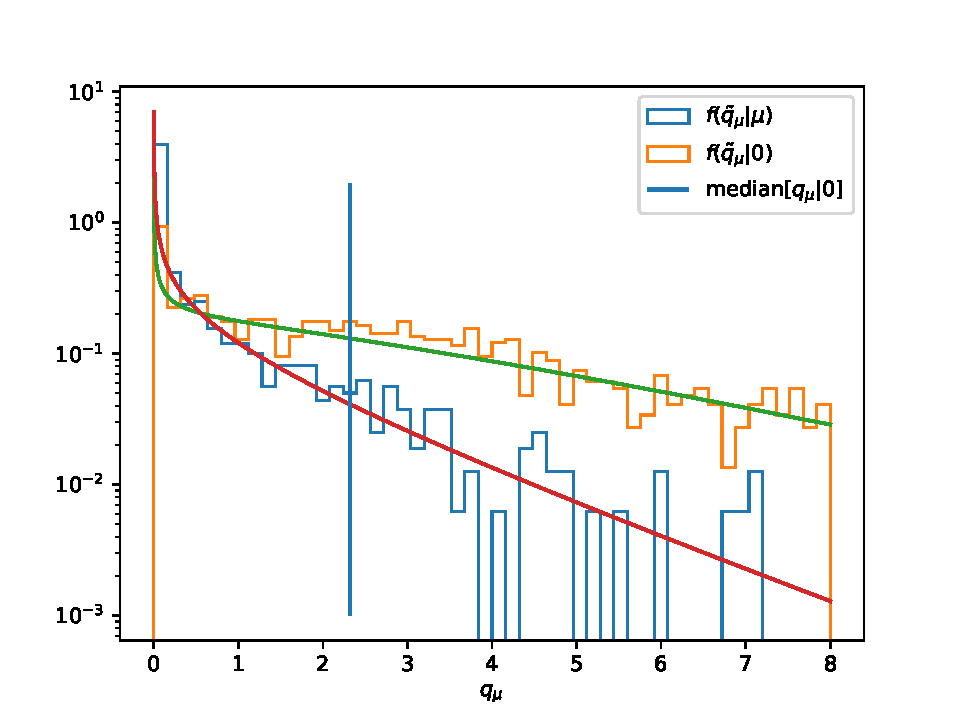
\includegraphics[width=\textwidth]{plots/median_plot.pdf}
    \end{minipage}
    \hfill
    \begin{minipage}{0.5\textwidth}
        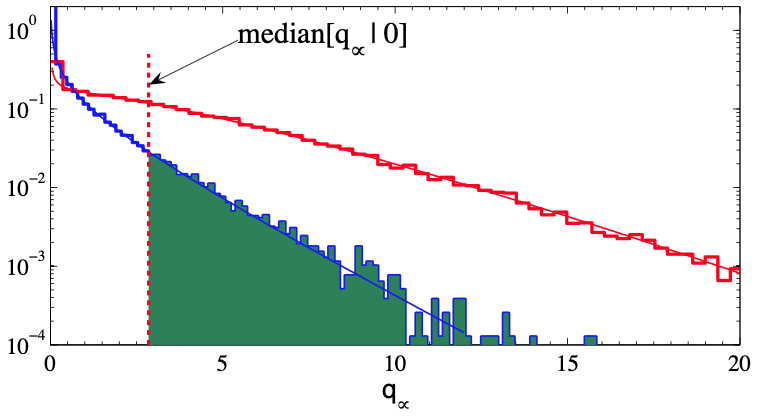
\includegraphics[width=\textwidth]{imgs/median.png}
    \end{minipage}
\end{frame}

\begin{frame}{Median-$1\sigma$}
    \Large
    \centering
    \begin{minipage}{0.49\textwidth}
        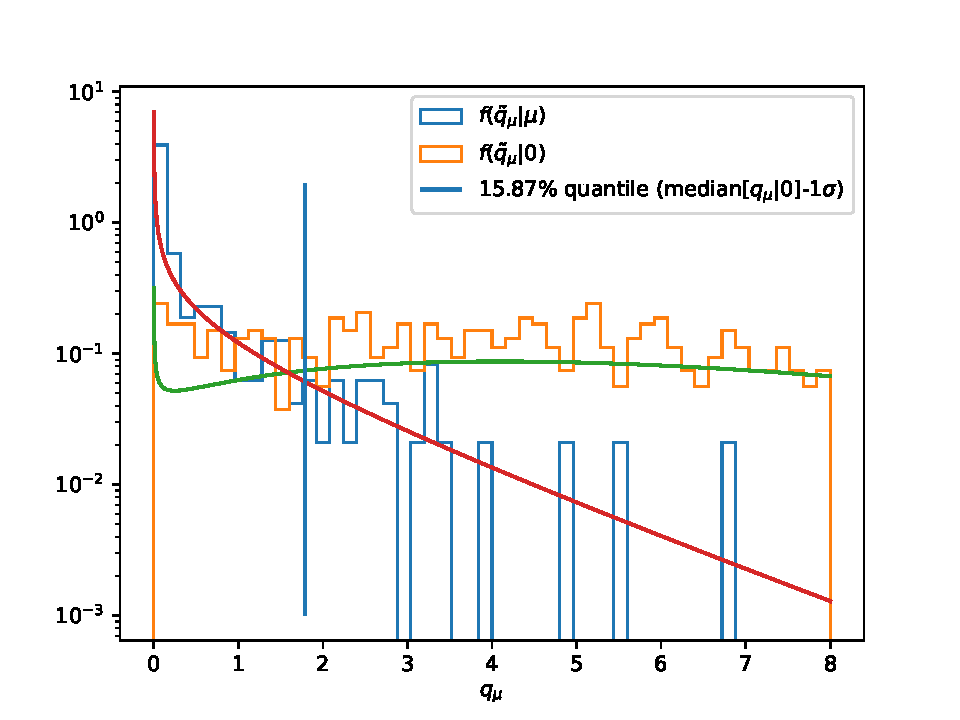
\includegraphics[width=\textwidth]{plots/sigma_plot.pdf}
    \end{minipage}
    \hfill
    \begin{minipage}{0.5\textwidth}
        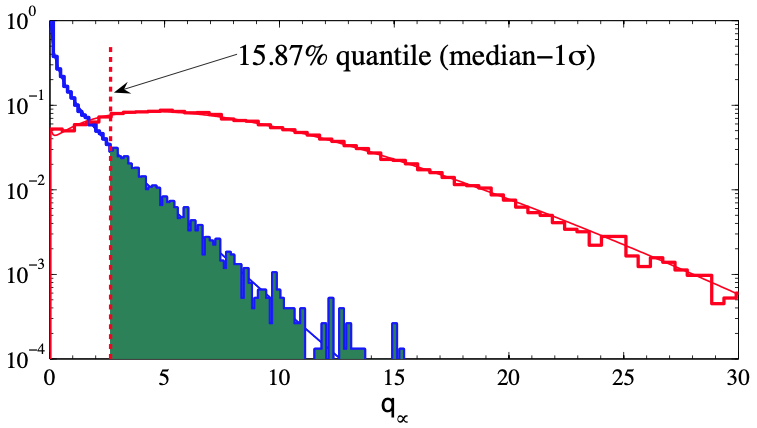
\includegraphics[width=\textwidth]{imgs/quantile.png}
    \end{minipage}
\end{frame}

\begin{frame}{Finally}
    \Large
    \centering
    \begin{minipage}{0.49\textwidth}
        \textbf{Finally:}
        \begin{itemize}
            \item UL data: $\mu_\text{up} = \hat{\mu} + \sigma\Phi^{-1}(1-\alpha)$
            \item Median: $med[\mu_\text{up}\vert\mu^\prime] = \mu^\prime + \sigma\Phi^{-1}(1-\alpha)$
            \item Band: $band_{N\sigma} = \mu^\prime + \sigma(\Phi^{-1}(1-\alpha)\pm N)$
        \end{itemize}
    \end{minipage}
    \hfill
    \begin{minipage}{0.5\textwidth}
        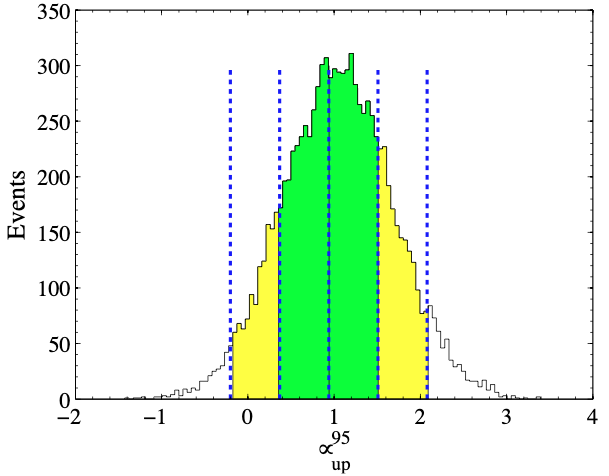
\includegraphics[width=\textwidth]{imgs/CL one mass.png}
    \end{minipage}
\end{frame}

\end{document}
